\documentclass[class=article, crop=false]{standalone}

\begin{document}
\section{Partie 4 - Observateur}
On ne dispose que de capteurs capables de donner les mesures de position $r(t)$ et $\theta(t)$. On va donc devoir construire un observateur asymptotique pour estimer l'intégralité de l'état. On pose:
\begin{equation}
    Y(t) = 
    \begin{bmatrix}
        y_1(t)\\
        y_2(t)\\
    \end{bmatrix}
    =
    \begin{bmatrix}
        x_1(t)\\
        x_3(t)\\
    \end{bmatrix}
    =
    \begin{bmatrix}
        r(t)\\
        \theta(t)\\
    \end{bmatrix}
\end{equation}
On s'intéresse toujours à l'équilibre associé à $r_{\text{ref}}$, Balle stabilisée sur l'axe de rotation du Plateau.

\newpage
\subsection{Question 18}
\begin{exercise}
    Montrer que le linéarisé tangent du système, avec mesure, autour de la position d'équilibre $r_{\text{ref}} = 0$ s'écrit:
    \begin{equation}
        \left\{
        \begin{aligned}
            \frac{\text{d}}{\text{dt}} 
            \underbrace{
            \begin{bmatrix}
                x_{1}(t)\\
                x_{2}(t)\\
                x_{3}(t)\\
                x_{4}(t)\\
            \end{bmatrix}}_{X(t)}
            &=
            \underbrace{
            \begin{bmatrix}
                0 & 1 & 0 & 0\\
                0 & 0 & -\frac{g}{1 + \sigma} & 0\\
                0 & 0 & 0 & 1\\
                -\frac{mg}{J_p} & 0 & 0 & 0\\
            \end{bmatrix}}_{A}
            \underbrace{
            \begin{bmatrix}
                x_{1}(t)\\
                x_{2}(t)\\
                x_{3}(t)\\
                x_{4}(t)\\
            \end{bmatrix}}_{X(t)}
            +
            \underbrace{
            \begin{bmatrix}
                0\\
                0\\
                0\\
                \frac{1}{J_p}\\
            \end{bmatrix}}_{B}
            \delta u(t)
            \\
            \underbrace{
            \begin{bmatrix}
                y_1(t)\\
                y_2(t)\\
            \end{bmatrix}}_{Y(t)}
            &=
            \underbrace{
            \begin{bmatrix}
                1 & 0 & 0 & 0\\
                0 & 0 & 1 & 0\\
            \end{bmatrix}}_{C}
            \underbrace{
            \begin{bmatrix}
                x_{1}(t)\\
                x_{2}(t)\\
                x_{3}(t)\\
                x_{4}(t)\\
            \end{bmatrix}}_{X(t)}
        \end{aligned}
        \right.
    \end{equation}
\end{exercise}
\begin{resolution}
    On considère la résolution faite sur (\ref{Q9}) Question 9 qui donne la première équation du système linéarise. Après on peut voir que avec la définition des états présenter sur (\ref{eq:def_states}) on a l'équation suivante:
    \begin{equation}
        \underbrace{
            \begin{bmatrix}
                y_1(t)\\
                y_2(t)\\
            \end{bmatrix}}_{Y(t)}
            =
            \underbrace{
            \begin{bmatrix}
                1 & 0 & 0 & 0\\
                0 & 0 & 1 & 0\\
            \end{bmatrix}}_{C}
            \underbrace{
            \begin{bmatrix}
                x_{1}(t)\\
                x_{2}(t)\\
                x_{3}(t)\\
                x_{4}(t)\\
            \end{bmatrix}}_{X(t)}
    \end{equation}
\end{resolution}

\newpage
\subsection{Question 19}
\begin{exercise}
    Le linéarisé tangent est-il observable? Vérifier le rang de la matrice d'observabilité avec MATLAB. On pourra également s'assurer que la matrice d'observabilité est bien conditionnée.
\end{exercise}
\begin{resolution}
    On note que le système sera Observable si et seulement si la Matrice de Observabilité $\mathcal{O}(A, C)$:
    \begin{equation}
        \boxed{
            \mathcal{O}(A, C) =
            \begin{bmatrix}
                C\\
                C\times A\\
                \vdots\\
                C\times A^{n-1}\\
            \end{bmatrix}
        }
    \end{equation}
    est de rang dim$(x)$, c'est-à-dire: si la matrice $\mathcal{O}(A, C)$ a une numéro de colognes linéairement indépendants égale à dimension du vecteur des états $x$, le système est observable.\\

    En utilisant le code suivant on calcule la matrice de Observabilité:
    \begin{scriptsize}\mycode
        \lstinputlisting[language=Matlab]{../src/Q19.m}
    \end{scriptsize}
    \begin{scriptsize}\mycode
        \begin{lstlisting}[language=Matlab]
>>>
success: system observable, rank 4

OBS =

    1.0000         0         0         0
         0         0    1.0000         0
         0    1.0000         0         0
         0         0         0    1.0000
         0         0   -5.4500         0
 -294.3000         0         0         0
         0         0         0   -5.4500
         0 -294.3000         0         0
        \end{lstlisting}
    \end{scriptsize}
    Le système est défini avec 4 états et, comme on peut voir avec le résultat du code, le rank de la matrice de commandabilité est aussi 4, car elle a quatre 4 colognes linéairement indépendants, donc le système est commandable.
\end{resolution}

\newpage
\subsection{Question 20}
\begin{exercise}
    Écrire les équations de l'observateur asymptotique permettant d'estimer l'état $X(t)$ à partir de la mesure $Y(t)$ et la commande $u(t)$. On notera $\hat{X}(t)$ l'état estimé de L le gain de l'observateur.
\end{exercise}
\begin{resolution}
    On considère l'équation suivante:
    \begin{equation}
        \dot{\hat{X}}(t) = A \cdot \hat{X}(t) + B \cdot u(t) + L \cdot (Y(t) - C \cdot \hat{X}(t))
    \end{equation}
    qui peut être implémente sur MATLAB avec le diagramme que suive:
    \begin{figure}[H]
        \centering
        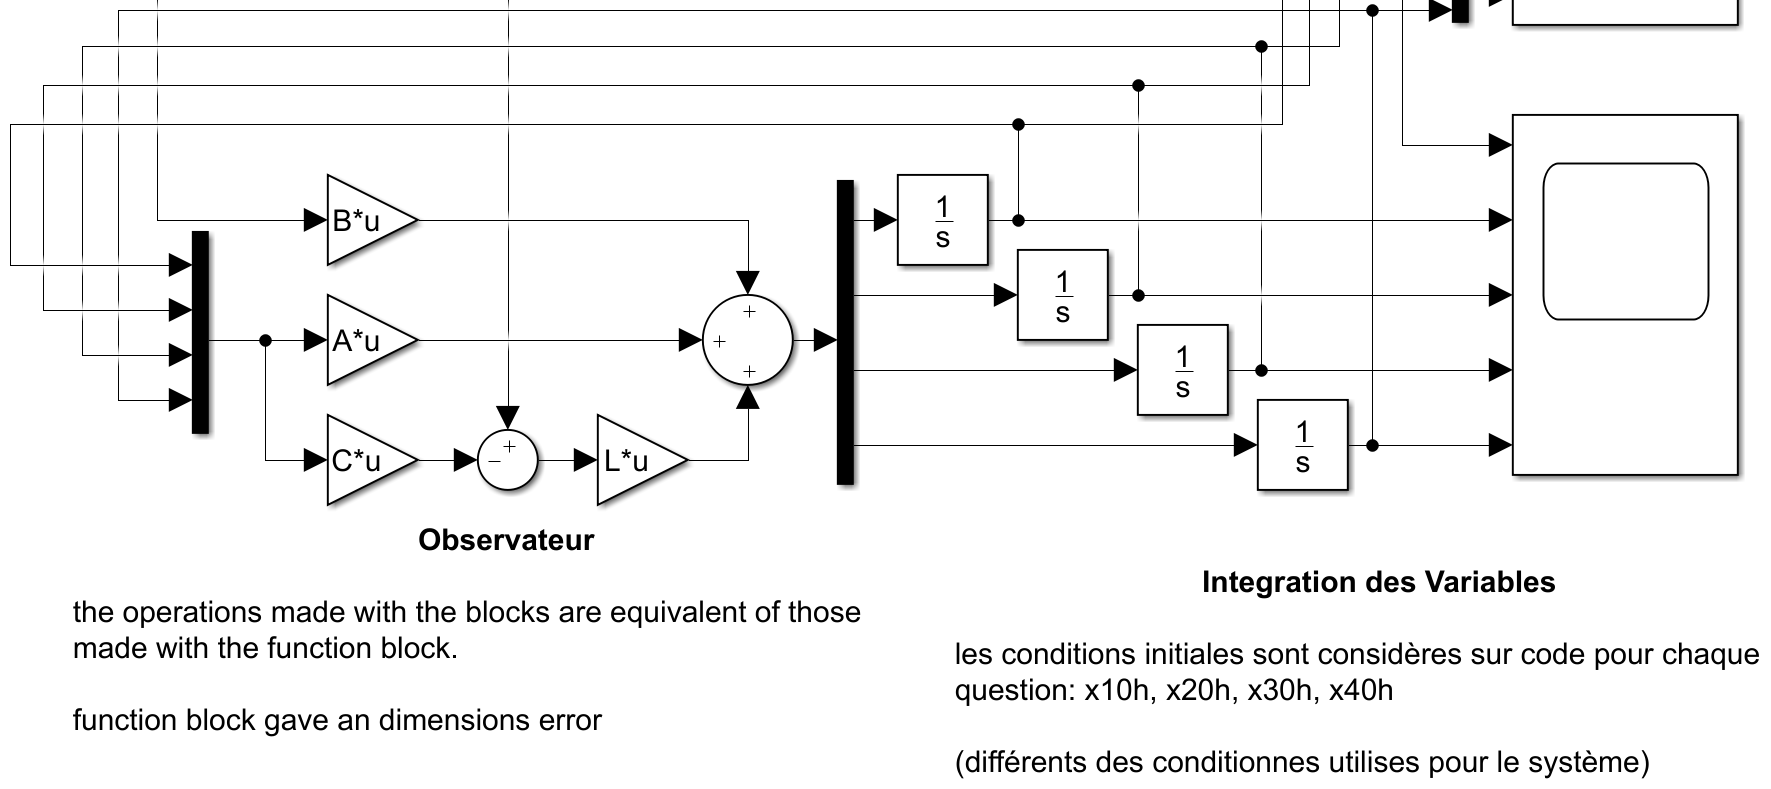
\includegraphics[width=0.75\textwidth]{../images/system_simulink_40.png}
        \caption{Système D'Intérêt Simulink, Observateur}
    \end{figure}
    On note que l'Observateur est représente avec des blocs basiques du Simulink. Un representation avec un bloc \texttt{function} sera une alternative valable mais l'équation serait différent.
\end{resolution}

\newpage
\subsection{Question 21}
On cherche à placer les valeurs de l'observateur en $-\omega$, $-3\omega$ et $-2\omega \pm i\omega$.
\begin{exercise}
    Calculer dans MATLAB le gain $L$ qui place les valeurs propres en boucle fermée sur les valeurs propres voulues. On pourra utiliser la fonction \href{https://www.mathworks.com/help/control/ref/place.html}{\texttt{place}}. Vérifier numériquement les valeurs propres de l'observateur avec MATLAB.
\end{exercise}
\begin{resolution}
    En utilisant le code suivant on boucle les valeurs propres sur les valeurs voulues:
    \begin{scriptsize}\mycode
        \lstinputlisting[language=Matlab]{../src/Q21.m}
    \end{scriptsize}
    \begin{scriptsize}\mycode
        \begin{lstlisting}[language=Matlab]
>>>
success: closed-loop pole assignment

L =

   23.9504    0.5651
  129.2383   22.7820
   -3.5660   26.6772
 -272.1502  190.9987
        \end{lstlisting}
    \end{scriptsize}
    Après on peut confirmer les valeurs propres sont en effet en boucle fermée avec l'équation suivante:
    \begin{equation}
        \det (A - L C - \lambda) = 0
    \end{equation}
    Comme on considère le système boucle fermée, c'est-à dire une système avec feedback, donc le $K$ n'est pas nulle, l'équation précédemment avec MATLAB on a:
    \begin{scriptsize}\mycode
        \begin{lstlisting}[language=Matlab]
>>> eig(A - L*C)

ans =
 -18.9853 + 0.0000i
  -6.3284 + 0.0000i
 -12.6569 + 6.3284i
 -12.6569 - 6.3284i
        \end{lstlisting}
    \end{scriptsize}
    Comme $\omega = 6.3284$ et on a défini les valeurs propres comme $-\omega$, $-3\omega$, $-2\omega\pm 1 i \omega$ le placement de pôles a bien marche.
\end{resolution}

\newpage
\subsection{Question 22}
\begin{exercise}
    Implémenter l'observateur dans le modèle Simulink. Vérifier qu'il permet bien d'estimer l'état au voisinage de la position $r_{\text{ref}} = 0$ avec un état suffisamment proche de l'équilibre pour que le linéarisé tangent reste une approximation valable.
\end{exercise}
\begin{resolution}
    L'Observateur complet peut être implémente avec le diagramme Simulink suivant:
    \begin{figure}[H]
        \centering
        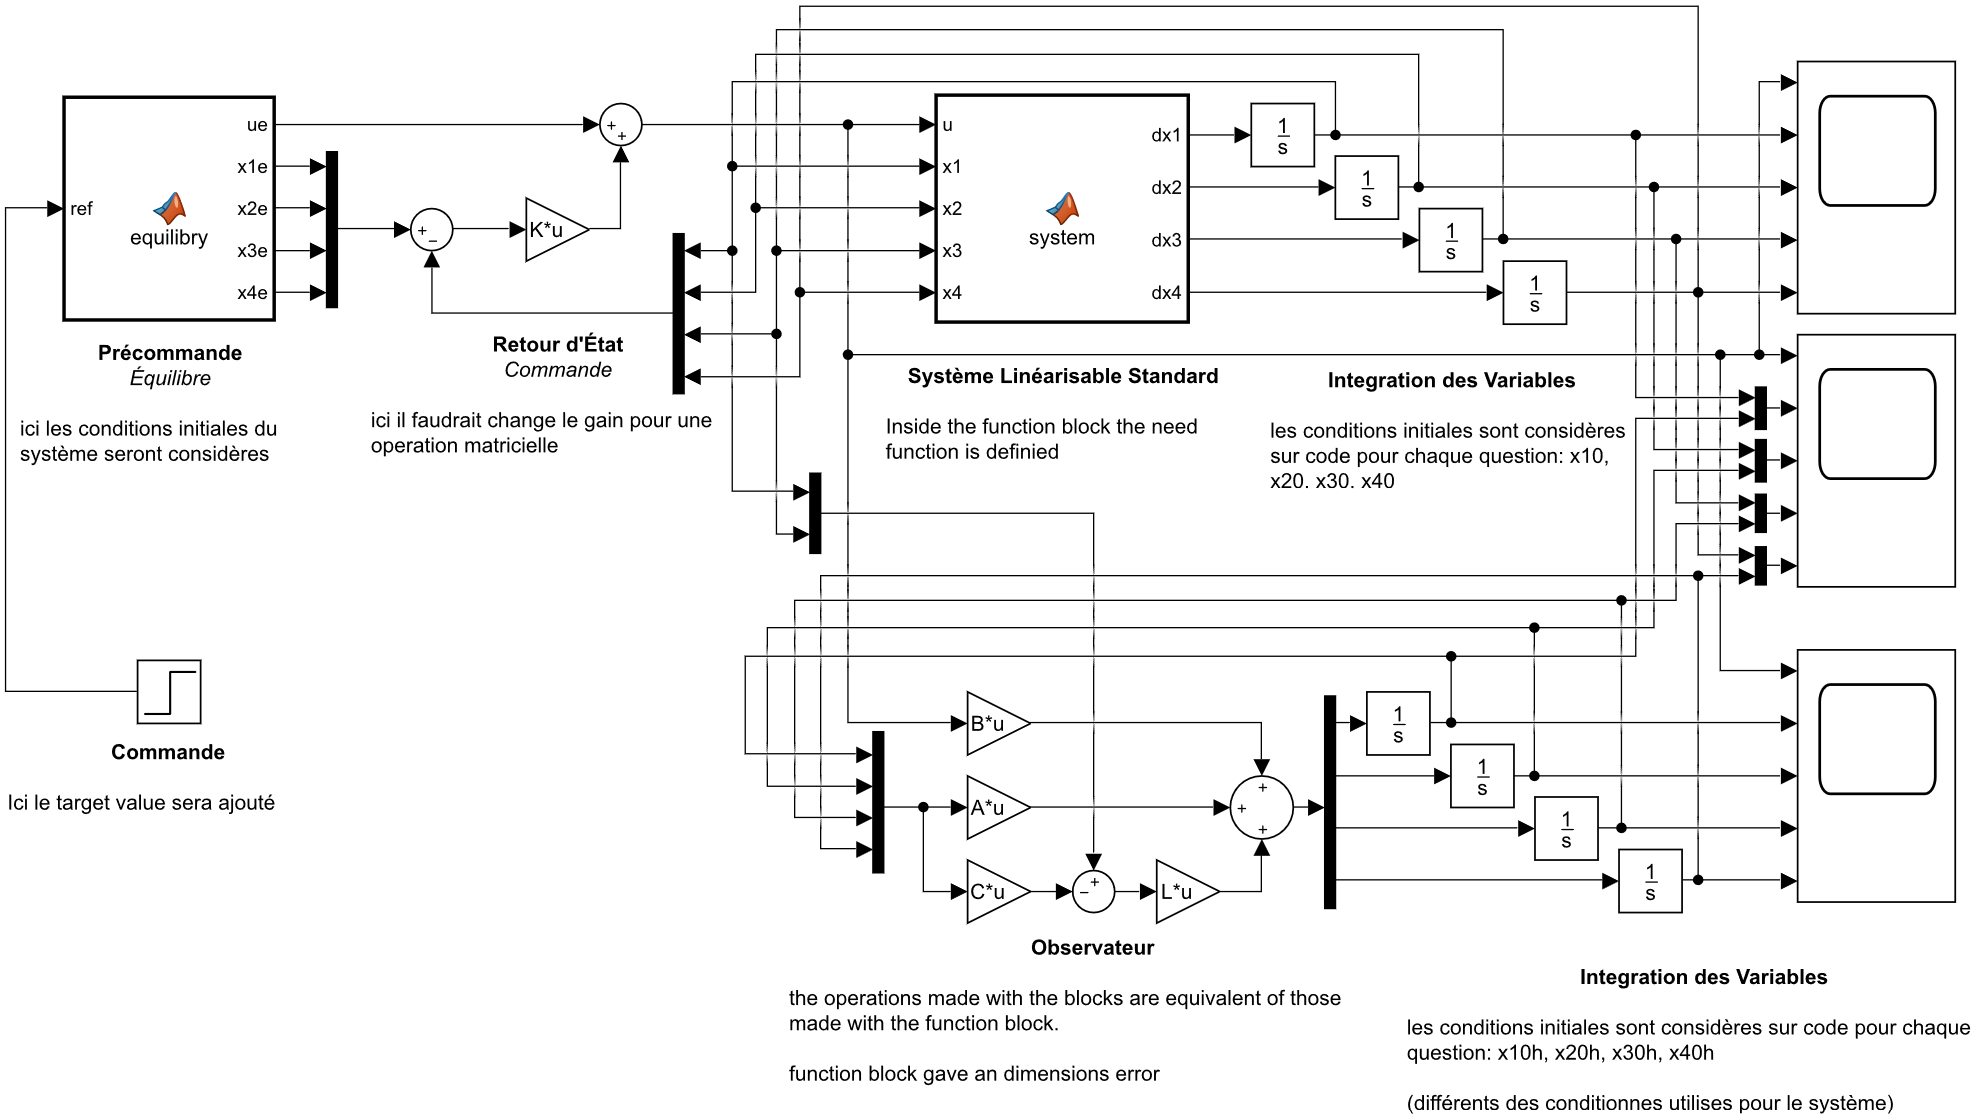
\includegraphics[width=0.75\textwidth]{../images/system_simulink_4.png}
        \caption{Système d'Intérêt Simulink, Observateur Complet}
    \end{figure}
    Qui donne les résultats suivants:
    \begin{figure}[H]
        \centering
        \begin{subfigure}[b]{0.45\textwidth}
            \centering
            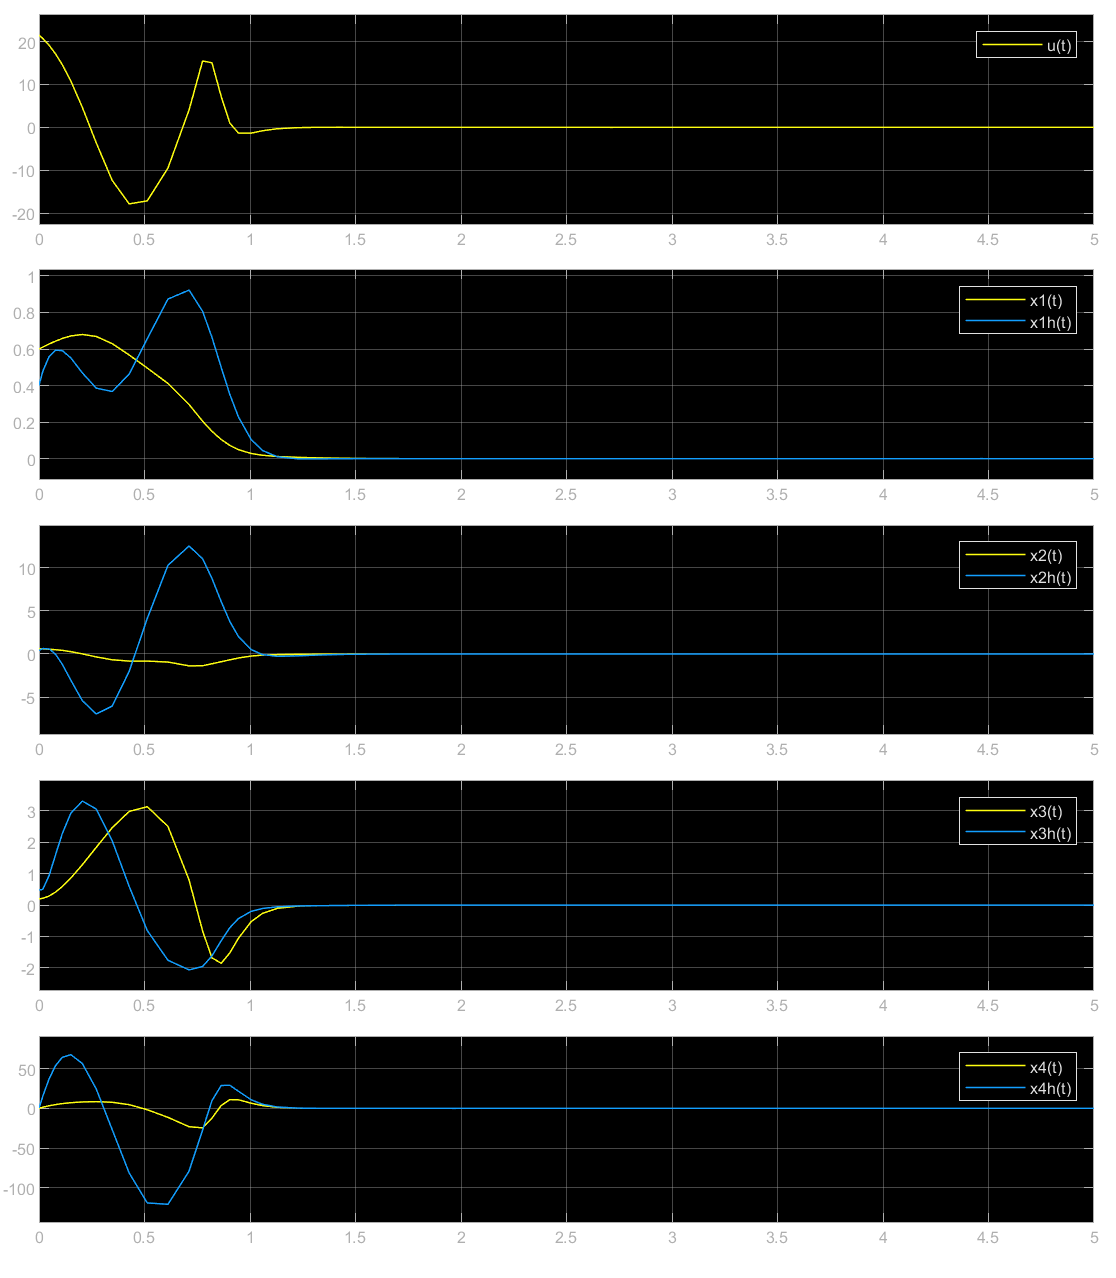
\includegraphics[width=\textwidth]{../images/m4_r0_s0.6_o0.4.png}
            \caption{$x_1(0) = x_2(0) = 0.6$}
        \end{subfigure}
        \begin{subfigure}[b]{0.45\textwidth}
            \centering
            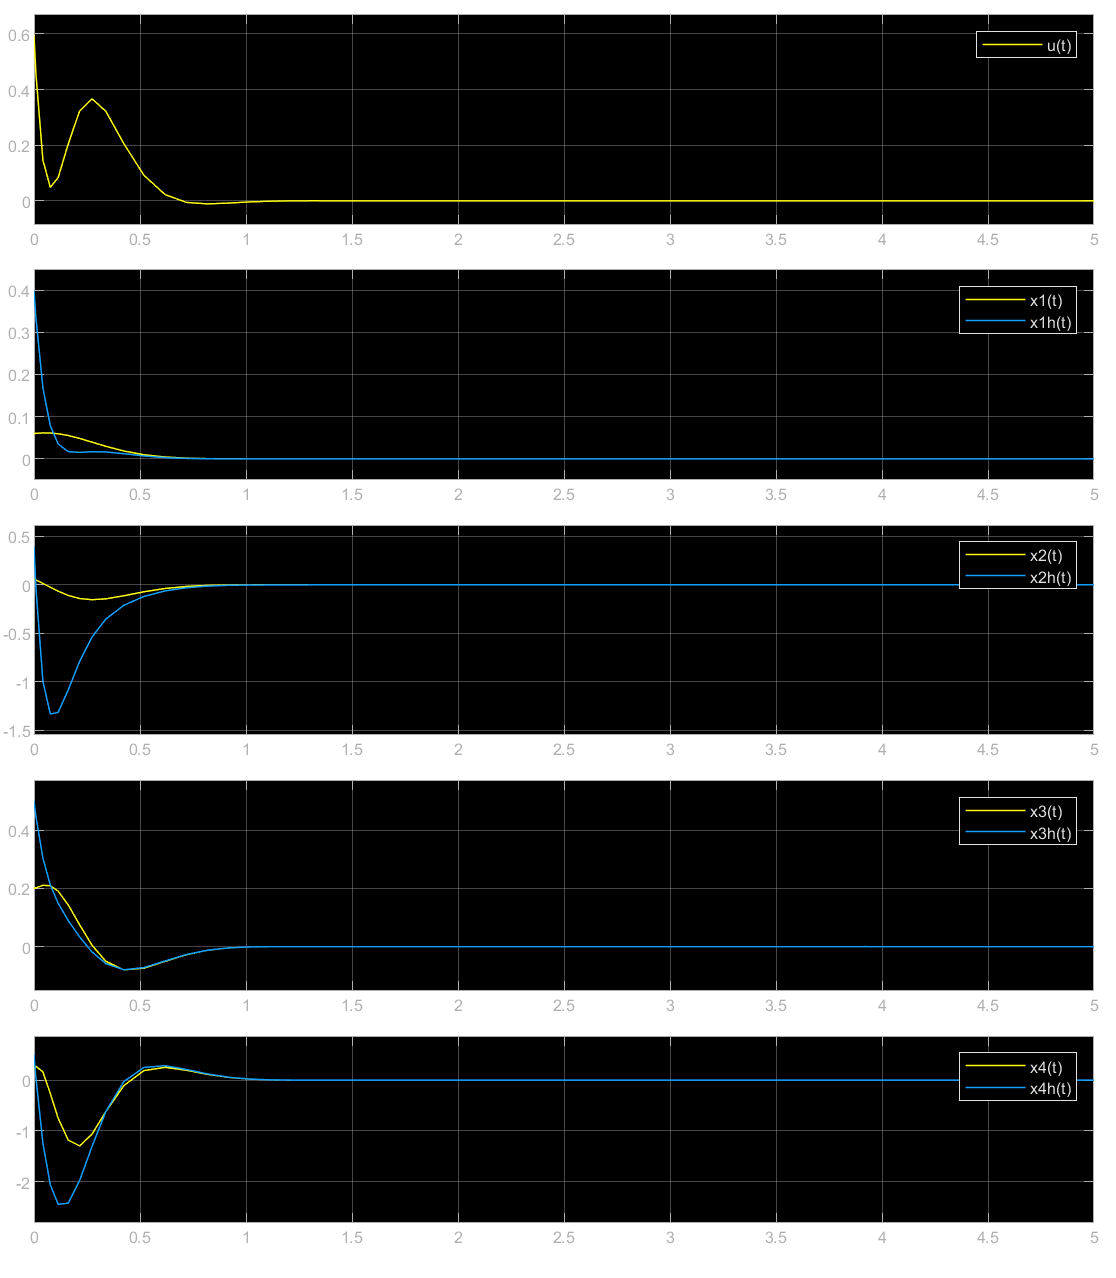
\includegraphics[width=\textwidth]{../images/m4_r0_s0.06_o0.4.png}
            \caption{$x_1(0) = x_2(0) = 0.06$}
        \end{subfigure}
        \caption{Simulation Observateur, autour de $r_{\text{ref}} = 0$}
    \end{figure}
    On considère $x_3(0) = x_4(0) = 0.2$, $\hat{x}_1(0) = \hat{x}_2(0) = 0.4$ et $\hat{x}_3(0) = \hat{x}_4(0) = 0.5$.
\end{resolution}
\end{document}